\documentclass{article}

\usepackage[
  a4paper,
  top=2cm,
  bottom=2cm,
  left=2.2cm,
  right=2.2cm
]{geometry}

\usepackage{csquotes}
\usepackage[hidelinks]{hyperref}
\usepackage{setspace}
\usepackage{fancyhdr}
\usepackage{xcolor}
\usepackage{soul}
\usepackage{amsmath}
\usepackage{amssymb}
\usepackage{mathtools}
\usepackage{braket}
\usepackage{colonequals}
\usepackage{amsopn}
\usepackage[version=4]{mhchem}
\usepackage{textcomp}
\usepackage{gensymb}
\usepackage{graphicx}
\usepackage{caption}
\usepackage{wrapfig}
\usepackage{tabularx}
\usepackage{booktabs}
\usepackage{multirow}
\usepackage{tikz} % we need to learn this one
\usepackage{parskip} % paragraph spcaing something...

% \usepackage{fontspec}
% \setmainfont{Inter}
% \setmainfont{Aptos}
% \setmainfont{Noto Sans}
\usetikzlibrary {shapes.geometric}

%%%%%%%%%%%%%%%%%%%%%%%%%%%%%%%%%%%%%%% tikzlibraries
\usetikzlibrary{
  arrows.meta,
  automata,
  positioning,
  shadows,
  mindmap,
  backgrounds,
  calendar,
  calc,
  topaths,
  intersections,
  graphs,
  quotes,
  fit
}

\title{NTMC Assignment Week 2}
\author{Anand}
\date{\today}

% ---- shorthand macros: everything is typeset in \mathtt, matching the paper's notation ----
\newcommand{\hf}[1]{\mathtt{h(}#1\mathtt{)}}          % hash function h(...)
\newcommand{\vt}[2]{\mathtt{#1}_{\mathtt{#2}}}         % a subscripted mathtt variable, e.g. \vt{RID}{DE_i}

%%%%%%%%%%%%%%%%%%%%%%%%%%%%%%%%%%%%%%%%%%%%%%%%%%%%%%%%%%%%%%%%%%%%%%%%%%%%%%%%%%%%%%%%%%%%%%%%%%%%%%%%%%%%%%%%%%%%%%%%%%%%%%%%%%%%%%%%%%%%%%%%%%%%%%%%%%%%%%%%%%%%%%
  % Document beigins %
%%%%%%%%%%%%%%%%%%%%%%%%%%%%%%%%%%%%%%%%%%%%%%%%%%%%%%%%%%%%%%%%%%%%%%%%%%%%%%%%%%%%%%%%%%%%%%%%%%%%%%%%%%%%%%%%%%%%%%%%%%%%%%%%%%%%%%%%%%%%%%%%%%%%%%%%%%%%%%%%%%%%%%

\begin{document}
\maketitle
\tableofcontents
\newpage

\section{Work for Week 2}

Technical Analysis \& Comparison
\begin{itemize}
  \item Explain workflow of the proposed protocol.
  \item Understand each phase of protocol.
  \item Analyze protocol, message flow, and security mechanisms.
  \item Study the implementation details and performance evaluations.
\end{itemize}

Proofs to submit:
\begin{itemize}
  \item Protocol flow diagram
  \item Step-by-step explaination of protocol
  \item Technical analysis report (2-3 pages)
\end{itemize}

\newpage

%%%%%%%%%%%%%%%%%%%%%%%%%%%%%%%%%%%%%%%%%%%%%%%%%%%%%%%%%%%%%%%%%%%%%%%%%%%%%%%%%%%%%%%%%%%%%%%%%%%%%%%%%%%%%%%%%%%%%%%%%%%%%%%%%%%%%%%%%%%%%%%%%%%%%%%%%%%%%%%%%%%%%%
  % Mind Map Start %
%%%%%%%%%%%%%%%%%%%%%%%%%%%%%%%%%%%%%%%%%%%%%%%%%%%%%%%%%%%%%%%%%%%%%%%%%%%%%%%%%%%%%%%%%%%%%%%%%%%%%%%%%%%%%%%%%%%%%%%%%%%%%%%%%%%%%%%%%%%%%%%%%%%%%%%%%%%%%%%%%%%%%%

\section{Protocol Mindmap}`

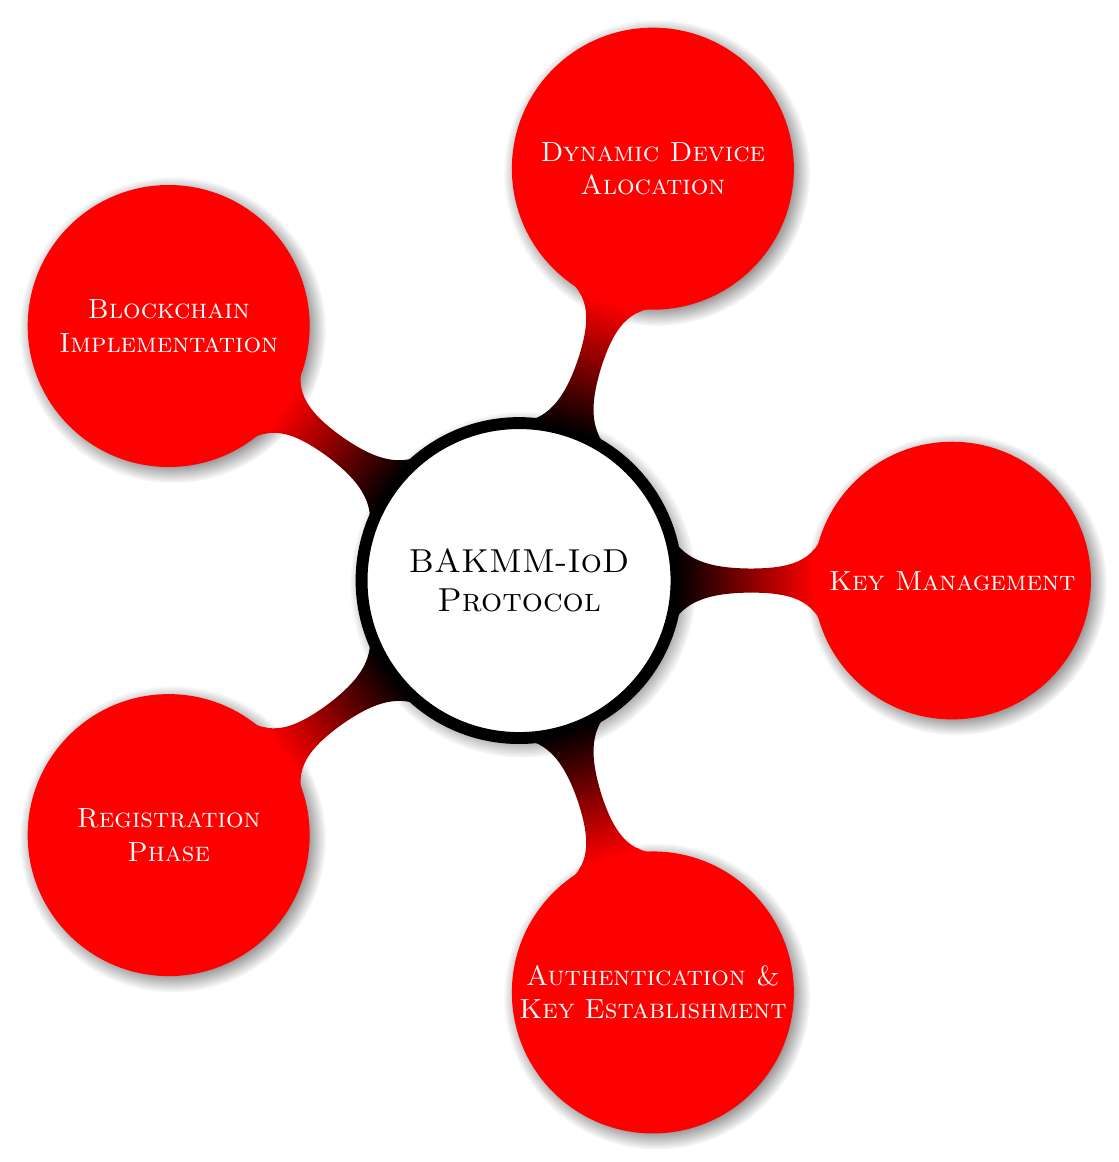
\begin{tikzpicture}
  [
    mindmap,
    grow cyclic,
    every node/.style={concept, circular drop shadow, text width=3.4cm, align=flush center},
    root concept/.append style={
      concept color=black,
      fill=white, line width=1ex,
      text=black, font=\large\scshape,
      xshift=5cm,
      yshift=-5cm
    },
    text=white,
    RP/.style={concept color=red},
    AK/.style={concept color=red},
    KM/.style={concept color=red},
    DA/.style={concept color=red},
    BI/.style={concept color=red},
    level 1/.append style={level distance=5.5cm,sibling angle=72,font=\scshape},
  ]
  % \draw[help lines] grid(10,10);
  \node [root concept] {BAKMM-IoD Protocol}
    child [RP] {node {Registration Phase}}
    child [AK] {node {Authentication \& Key Establishment}}
    child [KM] {node {Key Management}}
    child [DA] {node {Dynamic Device Alocation}}
    child [BI] {node {Blockchain Implementation}};
\end{tikzpicture}

%%%%%%%%%%%%%%%%%%%%%%%%%%%%%%%%%%%%%%%%%%%%%%% Tikz Set %%%%%%%%%%%%%%%%%%%%%%%%%%%%%%%%%%%%%%%%%%%%%%%%%%%%%%%%%%%%%%%%%%
% ---- colour palette (kept consistent across every diagram) ----
\definecolor{clrRA}{HTML}{2E2E38}      % registration authority / trust anchor
\definecolor{clrDE}{HTML}{C1440E}      % drone
\definecolor{clrES}{HTML}{1F6F78}      % ground station server
\definecolor{clrCS}{HTML}{5B3E8F}      % cloud server
\definecolor{clrChain}{HTML}{16537E}   % blockchain
\definecolor{clrSecure}{HTML}{2E8B57}  % secure channel (sea green)
\definecolor{clrOpen}{HTML}{808080}    % open / insecure channel
\definecolor{clrHash}{HTML}{B3282D}    % hash function h(.)
\definecolor{clrOp}{HTML}{1461A6}      % xor / concat / comparisons
\definecolor{clrMsg}{HTML}{8A5A00}     % message / macro labels M_i, m_i
\definecolor{clrKey}{HTML}{6A3D9A}     % session keys

\tikzset {
  entity/.style={text=white, rounded corners, draw=black, double},
  basic/.style={rounded corners, minimum width=2cm, align=left},
  random/.style={fill=pink!20, draw=red},
  fixed/.style={fill=teal!50, draw=black},
  random fixed/.style={fill=teal!10!pink, draw=brown},
  timestamp/.style={fill=cyan!10, draw=cyan},
  derived/.style={fill=yellow!20!white, draw=orange},
  actor/.style={
      minimum width=35mm,
      minimum height=10mm,
      align=center,
      font=\small\bfseries,
      line width=0.9pt
  },
  % --- entity variants, colour-coded per role, using mathtt labels ---
  entity RA/.style={entity, fill=clrRA, double=clrRA!40},
  entity DE/.style={entity, fill=clrDE, double=clrDE!40},
  entity ES/.style={entity, fill=clrES, double=clrES!40},
  entity CS/.style={entity, fill=clrCS, double=clrCS!40},
  % --- generic computation / verification panels ---
  compute/.style={basic, draw=clrDE!70!black, fill=clrDE!6, line width=0.7pt,
    font=\small, align=left, text width=8.6cm, drop shadow},
  compute alt/.style={basic, draw=clrES!70!black, fill=clrES!6, line width=0.7pt,
    font=\small, align=left, text width=12cm, drop shadow},
  compute third/.style={basic, draw=clrCS!70!black, fill=clrCS!6, line width=0.7pt,
    font=\small, align=left, text width=14cm, drop shadow},
  storebox/.style={fill=black!6, draw=black!25, rounded corners, line width=0.6pt},
  % --- channel arrows ---
  secure edge/.style={-{Stealth[length=3mm, round]}, thick, clrSecure, line width=1pt},
  open edge/.style={-{Stealth[length=3mm, round]}, thick, clrOpen, dashed, line width=0.9pt},
  open edge rev/.style={{Stealth[length=3mm, round]}-, thick, clrOpen, dashed, line width=0.9pt},
  derive edge/.style={-{Stealth[length=2.4mm, round]}, clrOp!70!black},
  % --- small badge to mark a channel as secure/insecure ---
  chanlabel secure/.style={font=\scriptsize\itshape, text=clrSecure},
  chanlabel open/.style={font=\scriptsize\itshape, text=clrOpen},
}
%%%%%%%%%%%%%%%%%%%%%%%%%%%%%%%%%%%%%%%%%%%%%%% Tikz Set %%%%%%%%%%%%%%%%%%%%%%%%%%%%%%%%%%%%%%%%%%%%%%%%%%%%%%%%%%%%%%%%%%

\newpage
\section{Protocl Flow Diagram}
\subsection{Registration Phase}

The registration is done offline, so communication is secure in this phase.

\subsubsection{Registraiion Authority Secrets Setup}

%%%%%%%%%%%%%%%%%%%%%%%%%%%%%%%%%%%%%%%%%%%%%%%%%%%%%%%%%%%%%%%%%%%%%%%%%%%%%%%%%%%%%%%%%%%%%%%%%%%%%%%%%%%%%%%%%%%%%%%%%%%%%%%%%%%%%%%%%%%%%%%%%%%%%%%%%%%%%%%%%%%%%%
  % Registration Authority Secrets Setup %
%%%%%%%%%%%%%%%%%%%%%%%%%%%%%%%%%%%%%%%%%%%%%%%%%%%%%%%%%%%%%%%%%%%%%%%%%%%%%%%%%%%%%%%%%%%%%%%%%%%%%%%%%%%%%%%%%%%%%%%%%%%%%%%%%%%%%%%%%%%%%%%%%%%%%%%%%%%%%%%%%%%%%%
\begin{tikzpicture}
  [
    >={Stealth[round,color=black!50]},
    every edge/.append style=dashed,
  ]
  % \draw [help lines] grid(17,24);
  \path node [actor, entity RA] (RA) {\texttt{RA}} 
    node [below right=10mm and -3mm of RA] [basic] [random] (SN) {$\mathtt{SN}_{\mathtt{RA}}$}
    node [right=of SN]       [basic] [random] (SK) {$\mathtt{k}_{\mathtt{RA}}$}
    node [right=of SK]       [basic] [fixed] (ID) {$\mathtt{ID}_{\mathtt{RA}}$}
    node [below=of SK]       [basic] [derived] (RID){$\mathtt{RID}_{\mathtt{RA}} = \mathtt{h(}\mathtt{ID}_{\mathtt{RA}}\parallel\mathtt{SN}_{\mathtt{RA}}\parallel\mathtt{K}_{\mathtt{RA}}\mathtt{)}$};
  \graph [edge quotes=near end] {
    {(SN), (SK), (ID)} -> (RID);
    (RA) -> [text=red,"\textit{generates}"] (SN);
    (RA) -> [text=red,"\textit{generates}"] (SK);
  };
  \begin{scope} [on background layer]
    \node [fill=black!10, fit=(SN) (SK) (ID) (RID), rounded corners] (memory) {};
    \node [below=1mm of memory, text=black!50] {\footnotesize in Registration Authority's memroy};
  \end{scope}
\end{tikzpicture}


\newpage
%%%%%%%%%%%%%%%%%%%%%%%%%%%%%%%%%%%%%%%%%%%%%%%%%%%%%%%%%%%%%%%%%%%%%%%%%%%%%%%%%%%%%%%%%%%%%%%%%%%%%%%%%%%%%%%%%%%%%%%%%%%%%%%%%%%%%%%%%%%%%%%%%%%%%%%%%%%%%%%%%%%%%%
  % Drone Registration %
%%%%%%%%%%%%%%%%%%%%%%%%%%%%%%%%%%%%%%%%%%%%%%%%%%%%%%%%%%%%%%%%%%%%%%%%%%%%%%%%%%%%%%%%%%%%%%%%%%%%%%%%%%%%%%%%%%%%%%%%%%%%%%%%%%%%%%%%%%%%%%%%%%%%%%%%%%%%%%%%%%%%%%
\subsubsection{Drone Registration}

\begin{figure}[ht]
\centering
\resizebox{\textwidth}{!}{%
\begin{tikzpicture}
  [
    >={Stealth[round,color=black!50]},
  ]
  \path
    node [actor, entity RA] (RA) {$\mathtt{RA}$}
    node [actor, entity DE] [right=10.6cm of RA] (DE) {$\vt{DE}{i}$};

  \path
    node [compute] [below=8mm of RA.south west, anchor=north west, text width=10cm] (calc)
      {
        Choose $\vt{ID}{DE_i}$, $\vt{k}{DE_i}$, $\vt{SN}{DE_i}$ for $\vt{DE}{i}$; note $\vt{RTS}{DE_i}$ \\[2pt]
        $\vt{RID}{DE_i} = \hf{\vt{RID}{RA}\parallel \vt{ID}{DE_i}\parallel \vt{k}{RA}\parallel \vt{k}{DE_i}\parallel \vt{SN}{DE_i}}$ \\[2pt]
        $\vt{TC}{DE_i} = \hf{\vt{RID}{RA}\parallel \vt{ID}{DE_i}\parallel \vt{k}{RA}\parallel \vt{k}{DE_i}\parallel \vt{SN}{DE_i}\parallel \vt{RTS}{DE_i}}$ \\[2pt]
        Generate provisional temporary identity $\vt{TID}{DE_i}$
      };

  \node [storebox, below=8mm of DE.south west, anchor=north west, text width=5.6cm, align=left, font=\small] (demem)
    {Stores in memory: \\
     $\{\vt{TID}{DE_i},\ \vt{RID}{DE_i},\ \vt{TC}{DE_i},\ \vt{MS}{DE_i-ES_j},\ \mathtt{h}(\cdot)\}$ \\[3pt]
     {\scriptsize\itshape $\vt{MS}{DE_i-ES_j}$: primary secret key shared with $\vt{ES}{j}$, unique per drone}};

  \path [draw, secure edge]
    (calc.east) -- (demem.west)
    node [midway, above, chanlabel secure] {registration bundle};
\end{tikzpicture}
}
\caption{Registration of drone $\vt{DE}{i}$ by the registration authority (RSDI1--RSDI2).}
\label{fig:drone-reg}
\end{figure}

\newpage
%%%%%%%%%%%%%%%%%%%%%%%%%%%%%%%%%%%%%%%%%%%%%%%%%%%%%%%%%%%%%%%%%%%%%%%%%%%%%%%%%%%%%%%%%%%%%%%%%%%%%%%%%%%%%%%%%%%%%%%%%%%%%%%%%%%%%%%%%%%%%%%%%%%%%%%%%%%%%%%%%%%%%%
  % Ground Station Server Registration %
%%%%%%%%%%%%%%%%%%%%%%%%%%%%%%%%%%%%%%%%%%%%%%%%%%%%%%%%%%%%%%%%%%%%%%%%%%%%%%%%%%%%%%%%%%%%%%%%%%%%%%%%%%%%%%%%%%%%%%%%%%%%%%%%%%%%%%%%%%%%%%%%%%%%%%%%%%%%%%%%%%%%%%
\subsubsection{Ground Station Server Registration}

\begin{figure}[ht]
\centering
\resizebox{\textwidth}{!}{%
\begin{tikzpicture}
  [
    >={Stealth[round,color=black!50]},
  ]
  \path
    node [actor, entity RA] (RA) {$\mathtt{RA}$}
    node [actor, entity ES] [right=10.6cm of RA] (ES) {$\vt{ES}{j}$};

  \path
    node [compute alt] [below=8mm of RA.south west, anchor=north west, text width=10cm] (calc)
      {
        Choose $\vt{k}{ES_j}$, $\vt{SN}{ES_j}$, $\vt{ID}{ES_j}$ for $\vt{ES}{j}$; note $\vt{RTS}{ES_j}$ \\[2pt]
        $\vt{RID}{ES_j} = \hf{\vt{RID}{RA}\parallel \vt{ID}{ES_j}\parallel \vt{k}{RA}\parallel \vt{k}{ES_j}\parallel \vt{SN}{ES_j}}$ \\[2pt]
        $\vt{TC}{ES_j} = \hf{\vt{RID}{RA}\parallel \vt{ID}{ES_j}\parallel \vt{k}{RA}\parallel \vt{k}{ES_j}\parallel \vt{SN}{ES_j}\parallel \vt{RTS}{ES_j}}$ \\[2pt]
        Generate provisional id number $\vt{TIN}{ES_j}$ and shared secret $\vt{MS}{ES_j-CS_k}$
      };

  \node [storebox, below=8mm of ES.south west, anchor=north west, text width=6.9cm, align=left, font=\small] (esmem)
    {Stores in secured database: \\
     $\{(\vt{TID}{DE_i}, \vt{RID}{DE_i}) \mid i=1,\ldots,n_{DE}\}$, \\
     $\vt{TIN}{ES_j},\ \vt{RID}{ES_j},\ \vt{TC}{ES_j}$, \\
     $\{\vt{MS}{DE_i-ES_j} \mid i=1,\ldots,n_{DE}\}$, $\vt{MS}{ES_j-CS_k}$, $\mathtt{h}(\cdot)$ \\[3pt]
     {\scriptsize\itshape $n_{DE}$: drones deployed under $\vt{ES}{j}$; the pairs $(\vt{TID}{DE_i}, \vt{RID}{DE_i})$ come from RA (Fig.~\ref{fig:drone-reg})}};

  \path [draw, secure edge]
    (calc.east) -- (esmem.west)
    node [midway, above, chanlabel secure] {registration bundle};
\end{tikzpicture}
}
\caption{Registration of ground station server $\vt{ES}{j}$ by the registration authority (RSES1--RSES2).}
\label{fig:es-reg}
\end{figure}

\newpage
%%%%%%%%%%%%%%%%%%%%%%%%%%%%%%%%%%%%%%%%%%%%%%%%%%%%%%%%%%%%%%%%%%%%%%%%%%%%%%%%%%%%%%%%%%%%%%%%%%%%%%%%%%%%%%%%%%%%%%%%%%%%%%%%%%%%%%%%%%%%%%%%%%%%%%%%%%%%%%%%%%%%%%
  % Cloud Server Registration %
%%%%%%%%%%%%%%%%%%%%%%%%%%%%%%%%%%%%%%%%%%%%%%%%%%%%%%%%%%%%%%%%%%%%%%%%%%%%%%%%%%%%%%%%%%%%%%%%%%%%%%%%%%%%%%%%%%%%%%%%%%%%%%%%%%%%%%%%%%%%%%%%%%%%%%%%%%%%%%%%%%%%%%
\subsubsection{Cloud Server Registration}

\begin{figure}[ht]
\centering
\resizebox{\textwidth}{!}{%
\begin{tikzpicture}
  [
    >={Stealth[round,color=black!50]},
  ]
  \path
    node [actor, entity RA] (RA) {$\mathtt{RA}$}
    node [actor, entity CS] [right=10.6cm of RA] (CS) {$\vt{CS}{k}$};

  \path
    node [compute third] [below=8mm of RA.south west, anchor=north west, text width=10cm] (calc)
      {
        Choose $\vt{k}{CS_k}$, $\vt{SN}{CS_k}$, $\vt{ID}{CS_k}$ for $\vt{CS}{k}$; note $\vt{RTS}{CS_k}$ \\[2pt]
        $\vt{RID}{CS_k} = \hf{\vt{RID}{RA}\parallel \vt{ID}{CS_k}\parallel \vt{k}{RA}\parallel \vt{k}{CS_k}\parallel \vt{SN}{CS_k}}$ \\[2pt]
        $\vt{TC}{CS_k} = \hf{\vt{RID}{RA}\parallel \vt{ID}{CS_k}\parallel \vt{k}{RA}\parallel \vt{k}{CS_k}\parallel \vt{SN}{CS_k}\parallel \vt{RTS}{CS_k}}$
      };

  \node [storebox, below=8mm of CS.south west, anchor=north west, text width=6.9cm, align=left, font=\small] (csmem)
    {Stores in secured database: \\
     $\{(\vt{TIN}{ES_j}, \vt{RID}{ES_j}) \mid j=1,\ldots,n_{ES}\}$, \\
     $\vt{RID}{CS_k},\ \vt{TC}{CS_k}$, \\
     $\{\vt{MS}{ES_j-CS_k} \mid j=1,\ldots,n_{ES}\}$, $\mathtt{h}(\cdot)$ \\[3pt]
     {\scriptsize\itshape $n_{ES}$: ground station servers deployed under $\vt{CS}{k}$}};

  \path [draw, secure edge]
    (calc.east) -- (csmem.west)
    node [midway, above, chanlabel secure] {registration bundle};
\end{tikzpicture}
}
\caption{Registration of cloud server $\vt{CS}{k}$ by the registration authority (RSCS1--RSCS2).}
\label{fig:cs-reg}
\end{figure}

\newpage
%%%%%%%%%%%%%%%%%%%%%%%%%%%%%%%%%%%%%%%%%%%%%%%%%%%%%%%%%%%%%%%%%%%%%%%%%%%%%%%%%%%%%%%%%%%%%%%%%%%%%%%%%%%%%%%%%%%%%%%%%%%%%%%%%%%%%%%%%%%%%%%%%%%%%%%%%%%%%%%%%%%%%%
  % Authentication Phase %
%%%%%%%%%%%%%%%%%%%%%%%%%%%%%%%%%%%%%%%%%%%%%%%%%%%%%%%%%%%%%%%%%%%%%%%%%%%%%%%%%%%%%%%%%%%%%%%%%%%%%%%%%%%%%%%%%%%%%%%%%%%%%%%%%%%%%%%%%%%%%%%%%%%%%%%%%%%%%%%%%%%%%%
\subsection{Authentication Phase}
\begin{figure} [ht]
\begin{tikzpicture}
  [
    >={Stealth[round,color=black!50]},
    every edge/.append style=dashed,
  ]
  % actors
  \path 
    node [actor] [entity DE] (de) {$\mathtt{DE}_i$\\Drone}
    node [actor] [entity ES] [right=10cm of de] (es) {$\mathtt{ES}_j$\\Ground Station};

  % life lines
  \draw[dashed, black!30] (de.south) -- ++(0,-15cm);
  \draw[dashed, black!30] (es.south) -- ++(0,-15cm);

  % de side
  \path 
    node [compute alt] [draw, fill=yellow!10] [font=\small] [below right=5mm and 0mm of de.south west] (c1)
      {
        Generate $\vt{rs}{1}$ and $\vt{T}{1}$ \\ 
        $
\vt{M}{1}
=
\hf{
    \vt{RID}{DE_i}
    \parallel
    \vt{MS}{DE_i-ES_j}
    \parallel
    \mathtt{T_1}
}
\mathtt{\oplus}
\hf{
    \mathtt{TC}_{\mathtt{DE_i}}
    \parallel
    \mathtt{rs_1}
    \parallel
    \vt{MS}{DE_i-ES_j}
    \parallel
    \mathtt{T_1}
}
$

$
\vt{M}{2}
=
\hf{
    \hf{
        \mathtt{TC}_{\mathtt{DE_i}}
        \parallel
        \mathtt{rs_1}
        \parallel
        \vt{MS}{DE_i-ES_j}
        \parallel
        \mathtt{T_1}
    }
    \parallel
    \vt{RID}{DE_i}
    \parallel
    \mathtt{T_1}
}
$
      }
    node [compute alt] [draw, fill=yellow!10] [font=\small] [below right=7.5cm and 0mm of de.south west] (c3)
      {
        $\left|\mathtt{T_2}-\mathtt{T_2^*}\right|\mathtt{\leq}\mathtt{\Delta T}$ \\
        $\mathtt{Create\ }\vt{SK}{DE_i,ES_j}^{\prime}$ \\
        $\mathtt{Check\ the\ session\ key\ using\ }\vt{M}{4}$ \\
        $\mathtt{If\ correct,\ set\ the\ new\ temporary\ identity\ from\ }\vt{M}{5}$ \\
        $\mathtt{Generate\ T_3}$ \\
        $\vt{M}{6}=\hf{\vt{SK}{DE_i,ES_j}\parallel\mathtt{T_3}}$
      }
    ;
 \path [draw]
   let \p1 = (de),
       \p2 = (c1.south),
       \p3 = (es)
  in
   (\x1, \y2-1cm) edge[open edge] node[above] [font=\small] {$MSG_1=\{TID_{DE_i}, M_1, M_2, T_1\}$} (\x3, \y2-1cm);

 \path [draw]
   let \p1 = (de),
       \p2 = (c3.south),
       \p3 = (es)
  in
   (\x1, \y2-1cm) edge[open edge] node[above] [font=\small] {$MSG_3=\{M_6, T_3\}$} (\x3, \y2-1cm);

   
  % es side
  \path 
    node [compute third] [draw=cyan, fill=cyan!10] [font=\small] [below left=3cm and 0mm of es.south east] (c2)
      {
        $\left|\mathtt{T_1}-\mathtt{T_1^*}\right|\mathtt{\leq}\mathtt{\Delta T}$ \\
$\mathtt{Create\ and\ check\ }\vt{M}{2}^{\prime}\mathtt{=}\vt{M}{2}$ \\
$\vt{M}{3}
=
\hf{
    \vt{RID}{DE_i}
    \mathtt{\parallel}
    \vt{MS}{DE_i-ES_j}
    \mathtt{\parallel}
    \mathtt{T_2}
}
\mathtt{\oplus}
\hf{
    \vt{RID}{ES_j}
    \mathtt{\parallel}
    \vt{TC}{ES_j}
    \mathtt{\parallel}
    \mathtt{rs_2}
    \mathtt{\parallel}
    \vt{MS}{DE_i-ES_j}
    \mathtt{\parallel}
    \mathtt{T_2}
}$ \\
$\vt{SK}{ES_j,DE_i}
=
\hf{
    \hf{
        \vt{TC}{DE_i}
        \mathtt{\parallel}
        \mathtt{rs_1}
        \mathtt{\parallel}
        \vt{MS}{DE_i-ES_j}
        \mathtt{\parallel}
        \mathtt{T_1}
    }
    \mathtt{\parallel}
    \hf{
        \vt{RID}{ES_j}
        \mathtt{\parallel}
        \vt{TC}{ES_j}
        \mathtt{\parallel}
        \mathtt{rs_2}
        \mathtt{\parallel}
        \vt{MS}{DE_i-ES_j}
        \mathtt{\parallel}
        \mathtt{T_2}
    }
    \mathtt{\parallel}
    \mathtt{T_1}
    \mathtt{\parallel}
    \mathtt{T_2}
    \mathtt{\parallel}
    \vt{RID}{DE_i}
    \mathtt{\parallel}
    \vt{MS}{DE_i-ES_j}
}$ \\
$\vt{M}{4}
=
\hf{
    \vt{SK}{ES_j,DE_i}
    \mathtt{\parallel}
    \mathtt{T_1}
    \mathtt{\parallel}
    \mathtt{T_2}
    \mathtt{\parallel}
    \vt{RID}{DE_i}
}$ \\
$\vt{M}{5}
=
\mathtt{TID}_{\mathtt{DE_i}}^{\mathtt{new}}
\mathtt{\oplus}
\hf{
    \hf{
        \vt{TC}{DE_i}
        \mathtt{\parallel}
        \mathtt{rs_1}
        \mathtt{\parallel}
        \vt{MS}{DE_i-ES_j}
        \mathtt{\parallel}
        \mathtt{T_1}
    }
    \mathtt{\parallel}
    \vt{RID}{DE_i}
    \mathtt{\parallel}
    \mathtt{T_2}
}$ 
      };
  \path 
    node [compute third] [draw=cyan, fill=cyan!10] [font=\small] [below left=11.5cm and 0mm of es.south east] (c4)
      {
        $\left|\mathtt{T_3}-\mathtt{T_3^*}\right|\mathtt{\leq}\mathtt{\Delta T}$ \\
$\mathtt{Create\ and\ check\ }\vt{M}{6}^{\prime}\mathtt{=}\vt{M}{6}$ 
      };
 \path [draw]
   let \p1 = (de),
       \p2 = (c2.south),
       \p3 = (es)
  in
   (\x1, \y2-1cm) edge[open edge rev] node[above] [font=\small] {$MSG_2=\{M_3,M_4,M_5,T_2\}$} (\x3, \y2-1cm);
\end{tikzpicture}
\caption{Authentication and session-key establishment between the drone and ground station server.}
\label{fig:de-es-auth}
\end{figure}

\newpage
%%%%%%%%%%%%%%%%%%%%%%%%%%%%%%%%%%%%%%%%%%%%%%%%%%%%%%%%%%%%%%%%%%%%%%%%%%%%%%%%%%%%%%%%%%%%%%%%%%%%%%%%%%%%%%%%%%%%%%%%%%%%%%%%%%%%%%%%%%%%%%%%%%%%%%%%%%%%%%%%%%%%%%
  % Key Management Phase %
%%%%%%%%%%%%%%%%%%%%%%%%%%%%%%%%%%%%%%%%%%%%%%%%%%%%%%%%%%%%%%%%%%%%%%%%%%%%%%%%%%%%%%%%%%%%%%%%%%%%%%%%%%%%%%%%%%%%%%%%%%%%%%%%%%%%%%%%%%%%%%%%%%%%%%%%%%%%%%%%%%%%%%
\subsection{Key Management Phase}

This procedure establishes the session key $\vt{SK}{ES_j,CS_k}$ shared between a ground station server and its cloud server, over the open channel (AKDEC1--AKDEC4).

\begin{figure}[ht]
\resizebox{\textwidth}{!}{%
\begin{tikzpicture}
  [
    >={Stealth[round,color=black!50]},
  ]
  \path
    node [actor, entity ES] (ES) {$\vt{ES}{j}$\\Ground Station}
    node [actor, entity CS] [right=10cm of ES] (CS) {$\vt{CS}{k}$\\Cloud Server};

  % --- ES side, step 1 ---
  \node [compute alt, below=6mm of ES.south west, anchor=north west] (c1)
    {
      Generate $\vt{TS}{1}$ and $\vt{RS}{1}$ \\
      $\textcolor{clrMsg}{m_1}=\hf{\vt{RID}{ES_j}\parallel \vt{MS}{ES_j-CS_k}\parallel \vt{TS}{1}} \textcolor{clrOp}{\oplus} \hf{\vt{TC}{ES_j}\parallel \vt{RS}{1}\parallel \vt{MS}{ES_j-CS_k}\parallel \vt{TS}{1}}$ \\
      $\textcolor{clrMsg}{m_2}=\hf{\hf{\vt{RS}{1}\parallel \vt{TC}{ES_j}\parallel \vt{MS}{ES_j-CS_k}\parallel \vt{TS}{1}} \parallel \vt{RID}{ES_j}\parallel \vt{MS}{ES_j-CS_k}\parallel \vt{TS}{1}}$
    };

  \path [draw]
   let \p1=(ES), \p2=(c1.south), \p3=(CS) in
   (\x1,\y2-1cm) edge[open edge] node[above, font=\small] {$msg_1=\{\vt{TIN}{ES_j}, m_1, m_2, \vt{TS}{1}\}$} (\x3,\y2-1cm);

  % --- CS side, step 2 (anchored to the bottom of c1, offset for the msg1 arrow) ---
  \node [compute third, anchor=north east, yshift=-1.8cm] at (CS.south east|-c1.south) (c2)
    {
      Check $\left|\vt{TS}{1}-\vt{TS}{1}^*\right|\textcolor{clrOp}{\le}\Delta T$; fetch $\vt{RID}{ES_j}, \vt{MS}{ES_j-CS_k}$ \\
      recompute $\hf{\vt{RS}{1}\parallel \vt{TC}{ES_j}\parallel \vt{MS}{ES_j-CS_k}\parallel \vt{TS}{1}}$ from $m_1$; check $m_2^{'}\textcolor{clrOp}{=}m_2$ \\
      Generate $\vt{TS}{2}$ and $\vt{RS}{2}$ \\
      $\textcolor{clrMsg}{m_3}=\hf{\vt{RS}{2}\parallel \vt{TC}{CS_k}\parallel \vt{MS}{ES_j-CS_k}\parallel \vt{TS}{2}} \textcolor{clrOp}{\oplus} \hf{\vt{RID}{ES_j}\parallel \vt{MS}{ES_j-CS_k}\parallel \vt{TS}{1}\parallel \vt{TS}{2}}$ \\
      $\textcolor{clrKey}{\vt{SK}{CS_k,ES_j}}=\hf{\hf{\vt{RS}{2}\parallel \vt{TC}{CS_k}\parallel \vt{MS}{ES_j-CS_k}\parallel \vt{TS}{2}} \parallel \hf{\vt{RS}{1}\parallel \vt{TC}{ES_j}\parallel \vt{MS}{ES_j-CS_k}\parallel \vt{TS}{1}} \parallel \vt{RID}{ES_j}\parallel \vt{MS}{ES_j-CS_k}\parallel \vt{TS}{1}\parallel \vt{TS}{2}}$ \\
      $\textcolor{clrMsg}{m_4}=\hf{\vt{SK}{CS_k,ES_j}\parallel \vt{RID}{ES_j}\parallel \vt{MS}{ES_j-CS_k}\parallel \vt{TS}{2}}$; generate $\vt{TIN}{ES_j}^{new}$ \\
      $\textcolor{clrMsg}{m_5}=\vt{TIN}{ES_j}^{new}\textcolor{clrOp}{\oplus} \hf{\vt{RID}{ES_j}\parallel \hf{\vt{RS}{1}\parallel \vt{TC}{ES_j}\parallel \vt{MS}{ES_j-CS_k}\parallel \vt{TS}{1}}\parallel \vt{TS}{2}}$
    };

  \path [draw]
   let \p1=(ES), \p2=(c2.south), \p3=(CS) in
   (\x1,\y2-1cm) edge[open edge rev] node[above, font=\small] {$msg_2=\{m_3,m_4,m_5,\vt{TS}{2}\}$} (\x3,\y2-1cm);

  % --- ES side, step 3 (anchored to the bottom of c2, offset for the msg2 arrow) ---
  \node [compute alt, anchor=north west, yshift=-1.8cm] at (ES.south west|-c2.south) (c3)
    {
      Check $\left|\vt{TS}{2}-\vt{TS}{2}^*\right|\textcolor{clrOp}{\le}\Delta T$ \\
      $\hf{\vt{RS}{2}\parallel \vt{TC}{CS_k}\parallel \vt{MS}{ES_j-CS_k}\parallel \vt{TS}{2}} = m_3 \textcolor{clrOp}{\oplus} \hf{\vt{RID}{ES_j}\parallel \vt{MS}{ES_j-CS_k}\parallel \vt{TS}{1}\parallel \vt{TS}{2}}$ \\
      $\textcolor{clrKey}{\vt{SK}{ES_j,CS_k}}=\hf{\hf{\vt{RS}{2}\parallel \vt{TC}{CS_k}\parallel \vt{MS}{ES_j-CS_k}\parallel \vt{TS}{2}} \parallel \hf{\vt{RS}{1}\parallel \vt{TC}{ES_j}\parallel \vt{MS}{ES_j-CS_k}\parallel \vt{TS}{1}} \parallel \vt{RID}{ES_j}\parallel \vt{MS}{ES_j-CS_k}\parallel \vt{TS}{1}\parallel \vt{TS}{2}}$ \\
      check $m_4^{'}\textcolor{clrOp}{=}m_4$; recover $\vt{TIN}{CS_k}^{new}$ from $m_5$; update $\vt{TIN}{ES_j}$ \\
      generate $\vt{TS}{3}$, $\textcolor{clrMsg}{m_6}=\hf{\vt{SK}{ES_j,CS_k}\parallel \vt{TS}{3}}$
    };

  \path [draw]
   let \p1=(ES), \p2=(c3.south), \p3=(CS) in
   (\x1,\y2-1cm) edge[open edge] node[above, font=\small] {$msg_3=\{m_6, \vt{TS}{3}\}$} (\x3,\y2-1cm);

  % --- CS side, step 4 (anchored to the bottom of c3, offset for the msg3 arrow) ---
  \node [compute third, anchor=north east, yshift=-1.8cm] at (CS.south east|-c3.south) (c4)
    {
      Check $\left|\vt{TS}{3}-\vt{TS}{3}^*\right|\textcolor{clrOp}{\le}\Delta T$ \\
      Check $m_6^{'}\textcolor{clrOp}{=}m_6$; if OK, $\vt{SK}{ES_j,CS_k}$ is confirmed correct
    };

  \coordinate (midbottom) at ($(ES.south east)!0.5!(CS.south west)$);
  \node [storebox, text width=11cm, font=\small, align=center, anchor=north]
    at ($(midbottom |- c4.south) + (0,-8mm)$)
    {both parties now hold the shared session key \\
    $\vt{SK}{ES_j,CS_k}\ (=\vt{SK}{CS_k,ES_j})$};

  \begin{scope}[on background layer]
    \draw[dashed, black!30] (ES.south) -- (ES.south|-c4.south);
    \draw[dashed, black!30] (CS.south) -- (CS.south|-c4.south);
  \end{scope}

\end{tikzpicture}
}
\caption{Key management between the ground station server and the cloud server.}
\label{fig:es-cs-keymgmt}
\end{figure}

\newpage
%%%%%%%%%%%%%%%%%%%%%%%%%%%%%%%%%%%%%%%%%%%%%%%%%%%%%%%%%%%%%%%%%%%%%%%%%%%%%%%%%%%%%%%%%%%%%%%%%%%%%%%%%%%%%%%%%%%%%%%%%%%%%%%%%%%%%%%%%%%%%%%%%%%%%%%%%%%%%%%%%%%%%%
  % Dynamic Device Addition Phase %
%%%%%%%%%%%%%%%%%%%%%%%%%%%%%%%%%%%%%%%%%%%%%%%%%%%%%%%%%%%%%%%%%%%%%%%%%%%%%%%%%%%%%%%%%%%%%%%%%%%%%%%%%%%%%%%%%%%%%%%%%%%%%%%%%%%%%%%%%%%%%%%%%%%%%%%%%%%%%%%%%%%%%%
\subsection{Dynamic Device Addition Phase}

New drones can be inducted into an already-deployed network without repeating the entire setup. As in registration, this bootstrapping is performed by the trusted RA and is transferred over a secure (offline) channel (DDA1--DDA2).

\begin{figure}[ht]
\centering
\resizebox{\textwidth}{!}{%
\begin{tikzpicture}
  [
    >={Stealth[round,color=black!50]},
  ]
  \node [actor, entity RA] (RA) {$\mathtt{RA}$};

  \node [compute, below=10mm of RA, text width=11.4cm, align=left] (calc)
    {
      Choose $\vt{ID}{DE_i}^{\nu}$, $\vt{k}{DE_i}^{\nu}$, $\vt{SN}{DE_i}^{\nu}$ for the new drone $\vt{DE}{i}^{\nu}$ \\[2pt]
      $\vt{RID}{DE_i}^{\nu} = \hf{\vt{RID}{RA}\parallel \vt{ID}{DE_i}^{\nu}\parallel \vt{k}{RA}\parallel \vt{k}{DE_i}^{\nu}\parallel \vt{SN}{DE_i}^{\nu}}$ \\[2pt]
      $\vt{TC}{DE_i}^{\nu} = \hf{\vt{RID}{RA}\parallel \vt{ID}{DE_i}^{\nu}\parallel \vt{k}{RA}\parallel \vt{k}{DE_i}^{\nu}\parallel \vt{SN}{DE_i}^{\nu}\parallel \vt{RTS}{DE_i}^{\nu}}$ \\[2pt]
      Generate temporary identity $\vt{TID}{DE_i}^{\nu}$
    };

  \node [actor, entity DE, below left=22mm and 16mm of calc.south] (DE) {$\vt{DE}{i}^{\nu}$};
  \node [actor, entity ES, below right=22mm and 16mm of calc.south] (ES) {$\vt{ES}{j}$};

  \node [storebox, below=6mm of DE, text width=5.6cm, align=left, font=\small] (demem)
    {Stores $\{\vt{TID}{DE_i}^{\nu},\ \vt{RID}{DE_i}^{\nu},\ \vt{TC}{DE_i}^{\nu},\ \vt{MS}{DE_i-ES_j}^{\nu},\ \mathtt{h}(\cdot)\}$ in its memory};

  \node [storebox, below=6mm of ES, text width=5.6cm, align=left, font=\small] (esmem2)
    {Updates its database with the registration info of $\vt{DE}{i}^{\nu}$};

  \path [draw, secure edge] (calc.south) -- +(0, -1cm) -| node [near start, above, chanlabel secure] {stores credentials} (DE.north);
  \path [draw, secure edge] (calc.south) -- +(0, -1cm) -| node [near start, above, chanlabel secure] {shares info} (ES.north);
  \path [draw, secure edge] (DE) -- (demem);
  \path [draw, secure edge] (ES) -- (esmem2);
\end{tikzpicture}
}
\caption{Dynamic addition of a new drone $\vt{DE}{i}^{\nu}$ to the network (DDA1--DDA2).}
\label{fig:dda}
\end{figure}

\newpage
%%%%%%%%%%%%%%%%%%%%%%%%%%%%%%%%%%%%%%%%%%%%%%%%%%%%%%%%%%%%%%%%%%%%%%%%%%%%%%%%%%%%%%%%%%%%%%%%%%%%%%%%%%%%%%%%%%%%%%%%%%%%%%%%%%%%%%%%%%%%%%%%%%%%%%%%%%%%%%%%%%%%%%
  % Blockchain Implementation Phase %
%%%%%%%%%%%%%%%%%%%%%%%%%%%%%%%%%%%%%%%%%%%%%%%%%%%%%%%%%%%%%%%%%%%%%%%%%%%%%%%%%%%%%%%%%%%%%%%%%%%%%%%%%%%%%%%%%%%%%%%%%%%%%%%%%%%%%%%%%%%%%%%%%%%%%%%%%%%%%%%%%%%%%%
\subsection{Blockchain Implementation Phase}

Once session keys have been established, drone data is relayed to the ground station server, packaged into a partial block, forwarded to the cloud server, assembled into a full block and finally committed to the consortium blockchain via consensus (BIP1--BIP3).

\begin{figure}[ht]
\centering
\resizebox{\textwidth}{!}{%
\begin{tikzpicture}
  [
    >={Stealth[round,color=black!50]},
  ]
  \path
    node [actor, entity DE] (DE) {$\vt{DE}{i}$}
    node [actor, entity ES] [right=5cm of DE] (ES) {$\vt{ES}{j}$}
    node [actor, entity CS] [right=5cm of ES] (CS) {$\vt{CS}{l}$};

  \path [draw, secure edge] (DE) -- node [midway, above, font=\scriptsize]
    {$\vt{Inf}{DE_i}$ via $\vt{SK}{DE_i,ES_j}$} (ES);
  \path [draw, secure edge] (ES) -- node [midway, above, font=\scriptsize]
    {$\vt{PBK}{ES_j}$ via $\vt{SK}{ES_j,CS_k}$} (CS);

  \node [compute alt, below=9mm of ES, xshift=-1.3cm, anchor=north, text width=8.3cm, align=left] (pbk)
    {
      \textbf{BIP1 --- partial block at $\vt{ES}{j}$:} \\
      Generate ECC key pair $\{\vt{KU}{ES_j}, \vt{KS}{ES_j}\}$; split $\vt{Inf}{DE_i}$ into $tr_x=\{tr_1,\ldots,tr_x\}$ \\
      $\vt{TR}{x} = E_{\vt{KU}{ES_j}}(tr_x)$ (ECC encryption) \\
      $\vt{PBK}{ES_j} = \{\vt{OWI}{ES_j},\ \vt{KU}{ES_j},\ \vt{TR}{x},\ \vt{MT}{root_{ES_j}}\}$
    };

  \node [compute third, below left=5cm and 0mm of CS.south east, anchor=north east, text width=8.6cm, align=left] (fbk)
    {
      \textbf{BIP2 --- full block at $\vt{CS}{l}$:} \\
      $\vt{FBK}{CS_l} = \{\vt{BID}{FBK_{CS_l}},\ \vt{RN}{FBK_{CS_l}},\ \vt{TSV}{FBK_{CS_l}},\ \vt{Hash}{FBK_{CS_l}},$ \\
      \hfill $\vt{Hash}{FBK_{CS_{l-1}}},\ \vt{OWI}{ES_j},\ \vt{KU}{ES_j},\ \vt{TR}{x},\ \vt{MT}{root_{ES_j}},\ \vt{Sign}{FBK_{CS_l}}\}$
    };

  \path [draw, derive edge] (pbk.south) -- (fbk.north);

  % blockchain visualisation: a small chain of committed blocks
  \node [entity CS, minimum width=27mm, minimum height=11mm, font=\scriptsize,
         below=3cm of fbk, xshift=-2.6cm] (blk1) {$\vt{FBK}{CS_{l-2}}$};
  \node [entity CS, minimum width=27mm, minimum height=11mm, font=\scriptsize,
         right=13mm of blk1] (blk2) {$\vt{FBK}{CS_{l-1}}$};
  \node [entity CS, minimum width=27mm, minimum height=11mm, font=\scriptsize,
         right=13mm of blk2] (blk3) {$\vt{FBK}{CS_l}$};

  \draw [-{Stealth[length=2.5mm, round]}, clrChain, thick] (blk1) -- node [above, font=\scriptsize] {hash link} (blk2);
  \draw [-{Stealth[length=2.5mm, round]}, clrChain, thick] (blk2) -- node [above, font=\scriptsize] {hash link} (blk3);
  \draw [-{Stealth[length=2.5mm, round]}, clrChain, thick, dashed] (fbk.south) to[out=270,in=90] (blk3.north);

  \begin{scope}[on background layer]
    \node [storebox, fill=clrChain!8, draw=clrChain!60, fit=(blk1)(blk2)(blk3), inner sep=4mm,
           label={[font=\small\bfseries, text=clrChain]above:consortium blockchain $\vt{BCH}{IoD_i}$}] {};
  \end{scope}

  \node [below=4mm of blk3, text width=7.2cm, align=center, font=\scriptsize, text=black!55]
    {\textbf{BIP3:} leader $\vt{CS}{l}^{\prime\prime}$ runs pBFT consensus over $\vt{FBK}{CS_l}$; on success it is committed to $\vt{BCH}{IoD_i}$};
\end{tikzpicture}
}
\caption{Blockchain implementation phase: from drone data to a committed block (BIP1--BIP3).}
\label{fig:blockchain}
\end{figure}


\newpage
% Requires only: \usepackage{booktabs}
% All protocol identifiers are typeset using \texttt{} as requested.

\subsection{Technical Analysis of the BAKMM-IoD Protocol}
\label{subsec:technical-analysis-bakmm}

The BAKMM-IoD protocol consists of five major stages: registration, authentication
and key establishment, key management, dynamic device addition, and blockchain
formation. The registration and dynamic-device stages are trusted provisioning
operations, whereas the authentication and key-management stages are open-channel
cryptographic exchanges that can be represented directly in SPDL and verified using
Scyther. The paper explicitly describes the authentication phase as a three-message
exchange and the key-management phase as another three-message exchange. The
Scyther implementation uses \texttt{send}, \texttt{recv}, and the security claims
\texttt{Secret}, \texttt{Alive}, \texttt{Weakagree}, \texttt{Niagree}, and
\texttt{Nisynch}. The corrected SPDL models additionally represent the equality
checks in the protocol by using the expected cryptographic expressions directly as
receive patterns. This is important because an unconstrained declaration such as
\texttt{var m4} followed by \texttt{recv(...,m4,...)} does not model the protocol's
actual check \texttt{m4'}=\texttt{m4}.

\subsubsection{Registration and Credential Provisioning}

During registration, the trusted registration authority \texttt{RA} generates the
long-term credentials and derives pseudo-identities and temporal credentials. For a
drone \texttt{DEi}, the principal values are \texttt{RIDDEi} and \texttt{TCDEi};
for a ground station server \texttt{ESj}, they are \texttt{RIDESj} and
\texttt{TCESj}; and for a cloud server \texttt{CSk}, they are \texttt{RIDCSk} and
\texttt{TCCSk}. Each pseudo-identity requires one hash operation and each temporal
credential requires one additional hash operation. The common value
\texttt{RIDRA} is computed once as one hash operation. Consequently, the complete
registration of one \texttt{DEi}, one \texttt{ESj}, and one \texttt{CSk} requires
seven hash evaluations when \texttt{RIDRA} is included once:
three for \texttt{DEi}, two for \texttt{ESj}, and two for \texttt{CSk}.

Registration is not treated as an open-channel transaction in the SPDL model,
because the paper describes it as trusted provisioning and secure storage rather
than as an adversarial message exchange. Therefore its communication length is
not assigned a fabricated bit count. The corresponding SPDL file
\texttt{01\_registration.spdl} models the credential derivation computations only.

\begin{table}[ht]
\centering
\caption{Registration computation cost.}
\label{tab:bakmm-registration-cost}
\begin{tabular}{llll}
\toprule
Entity & Operation & Hash evaluations & Average server time \\
\midrule
\texttt{RA} & \texttt{RIDRA} & 1 & 0.055 ms \\
\texttt{DEi} provisioning & \texttt{RIDDEi}, \texttt{TCDEi} & 2 & 0.110 ms \\
\texttt{ESj} provisioning & \texttt{RIDESj}, \texttt{TCESj} & 2 & 0.110 ms \\
\texttt{CSk} provisioning & \texttt{RIDCSk}, \texttt{TCCSk} & 2 & 0.110 ms \\
\midrule
Total & & 7 & 0.385 ms \\
\bottomrule
\end{tabular}
\end{table}

The timing in Table~\ref{tab:bakmm-registration-cost} uses the average one-way
hash execution time \texttt{Th}=0.055 ms measured under the server platform
reported in the paper. The corresponding Raspberry Pi 3 average is
\texttt{Th}=0.309 ms.

\subsubsection{Authentication and Key Establishment}

The authentication phase establishes a common session key between \texttt{DEi} and
\texttt{ESj}. The three exchanged messages are

\begin{align}
\texttt{MSG1} &= \{\texttt{TIDDEi},\texttt{M1},\texttt{M2},\texttt{T1}\},\\
\texttt{MSG2} &= \{\texttt{M3},\texttt{M4},\texttt{M5},\texttt{T2}\},\\
\texttt{MSG3} &= \{\texttt{M6},\texttt{T3}\}.
\end{align}

The protocol uses fresh values \texttt{rs1}, \texttt{rs2}, \texttt{T1},
\texttt{T2}, and \texttt{T3}. The first message authenticates the drone through
\texttt{M2}. The second message provides the server contribution \texttt{rs2},
the session-key confirmation value \texttt{M4}, and the updated temporary
identity protected by \texttt{M5}. Finally, \texttt{M6} confirms to the ground
station server that the drone derived the same session key.

The session key is

\begin{equation}
\texttt{SKDEiESj} =
\texttt{h(h(TCDEi,rs1,MSDEiESj,T1),
h(RIDESj,TCESj,rs2,MSDEiESj,T2),
T1,T2,RIDDEi,MSDEiESj)}.
\end{equation}

For the communication-cost calculation, the paper assumes an identity and a
random number occupy 160 bits, an ECC point occupies 320 bits, a SHA-256 hash
occupies 256 bits, and a timestamp occupies 32 bits. Hence,

\begin{align}
L_{\texttt{MSG1}}
 &=160+256+256+32
 =704~\text{bits},\\
L_{\texttt{MSG2}}
 &=256+256+160+32
 =704~\text{bits},\\
L_{\texttt{MSG3}}
 &=256+32
 =288~\text{bits}.
\end{align}

Thus, direct calculation from the field sizes stated in the paper gives

\begin{equation}
L_{\mathrm{auth}}=704+704+288=1696~\text{bits}.
\end{equation}

The paper's comparative communication table reports a total of 1792 bits for
BAKMM-IoD. Therefore, there is a 96-bit discrepancy between the published total
and the direct calculation from the published field-size assumptions. The
reported value should not be silently substituted into the individual message
lengths; both values should be documented when reproducing the paper's analysis.

\begin{table}[ht]
\centering
\caption{Authentication message size and computation cost.}
\label{tab:bakmm-auth-cost}
\begin{tabular}{llllll}
\toprule
Message & Direction & Length & Sender hashes & Receiver hashes &
Purpose \\
\midrule
\texttt{MSG1} & \texttt{DEi}\rightarrow\texttt{ESj}
& 704 bits & 4 & 2 & Drone authentication \\
\texttt{MSG2} & \texttt{ESj}\rightarrow\texttt{DEi}
& 704 bits & 8 & 8 & Key establishment and server authentication \\
\texttt{MSG3} & \texttt{DEi}\rightarrow\texttt{ESj}
& 288 bits & 1 & 1 & Session-key confirmation \\
\midrule
Total & & 1696 bits & 13 & 11 & \\
\bottomrule
\end{tabular}
\end{table}

The sender-side hash counts are obtained directly from the equations. For
example, \texttt{DEi} evaluates two hashes for \texttt{M1}, two for
\texttt{M2}, three for the session key, and one for \texttt{M6}, giving
\texttt{8Th}. Similarly, \texttt{ESj} evaluates two hashes for \texttt{M3},
three for the session key, one for \texttt{M4}, and two for \texttt{M5}, also
giving \texttt{8Th}. This agrees with the paper's reported computation-cost
expression of approximately \texttt{8Th} per endpoint.

The receiver-side verification work is separate from the paper's simplified
\texttt{8Th} accounting. In particular, verification and recovery operations
introduce additional hash evaluations. Therefore, for a complete implementation
cost estimate, the verification computations should be included in addition to
the published sender-side estimate.

Using the paper's average execution times,
\texttt{Th}=0.055 ms on the server and \texttt{Th}=0.309 ms on Raspberry Pi 3,
the published \texttt{8Th} estimate corresponds to approximately
0.44 ms on the server and 2.47 ms on the Raspberry Pi 3.

\subsubsection{Key Management Between \texttt{ESj} and \texttt{CSk}}

The key-management phase follows the same three-message structure:

\begin{align}
\texttt{MSG1} &= \{\texttt{TINESj},\texttt{m1},\texttt{m2},\texttt{TS1}\},\\
\texttt{MSG2} &= \{\texttt{m3},\texttt{m4},\texttt{m5},\texttt{TS2}\},\\
\texttt{MSG3} &= \{\texttt{m6},\texttt{TS3}\}.
\end{align}

The session key is

\begin{equation}
\texttt{SKESjCSk} =
\texttt{h(h(RS2,TCCSk,MSESjCSk,TS2),
h(RS1,TCESj,MSESjCSk,TS1),
RIDESj,MSESjCSk,TS1,TS2)}.
\end{equation}

The message structure is analogous to the authentication phase. Under the same
field-size assumptions, the three messages have lengths

\begin{align}
L_{\texttt{MSG1}} &=160+256+256+32=704~\text{bits},\\
L_{\texttt{MSG2}} &=256+256+160+32=704~\text{bits},\\
L_{\texttt{MSG3}} &=256+32=288~\text{bits}.
\end{align}

Consequently, the calculated communication overhead is again

\begin{equation}
L_{\mathrm{KM}}=1696~\text{bits}.
\end{equation}

The paper does not provide a separate communication-cost entry for the
\texttt{ESj}-\texttt{CSk} key-management exchange; therefore this 1696-bit value
is a derived value based on the published field-size assumptions.

\begin{table}[ht]
\centering
\caption{Key-management message size and computation cost.}
\label{tab:bakmm-keymgmt-cost}
\begin{tabular}{llllll}
\toprule
Message & Direction & Length & Sender hashes & Receiver hashes &
Purpose \\
\midrule
\texttt{MSG1} & \texttt{ESj}\rightarrow\texttt{CSk}
& 704 bits & 4 & 2 & ES authentication \\
\texttt{MSG2} & \texttt{CSk}\rightarrow\texttt{ESj}
& 704 bits & 8 & 5 & Key establishment and confirmation \\
\texttt{MSG3} & \texttt{ESj}\rightarrow\texttt{CSk}
& 288 bits & 1 & 1 & Session-key confirmation \\
\midrule
Total & & 1696 bits & 13 & 8 & \\
\bottomrule
\end{tabular}
\end{table}

The sender-side generation cost is therefore \texttt{9Th} for \texttt{ESj} when
all its key-management values are generated, and \texttt{8Th} for \texttt{CSk}.
The additional receiver-side verification consists of two hashes for the
\texttt{MSG1} verification, five hashes for \texttt{MSG2} verification and one
hash for \texttt{MSG3} verification. Thus, the full symbolic computation count
is higher than the sender-only count. The sender-side total is
\texttt{17Th}, whereas including the receiver-side verification gives
\texttt{25Th}.

\subsubsection{Dynamic Device Addition}

The dynamic-device addition phase allows a new drone \texttt{DEv} to be added
without redesigning the complete network. The registration authority generates
\texttt{IDDEv}, \texttt{kDEv}, and \texttt{SNDEv}, then derives
\texttt{RIDDEv} and \texttt{TCDEv}. If \texttt{RIDRA} is already available, the
addition requires two new hash evaluations:

\begin{align}
\texttt{RIDDEv} &=
\texttt{h(RIDRA,IDDEv,kRA,kDEv,SNDEv)},\\
\texttt{TCDEv} &=
\texttt{h(RIDRA,IDDEv,kRA,kDEv,SNDEv,RTSDEv)}.
\end{align}

Hence the computational overhead is approximately \texttt{2Th}, corresponding
to 0.110 ms on the reported server platform or 0.618 ms on Raspberry Pi 3.
The paper describes the subsequent sharing of the registration information
with deployed ground-station servers as secure provisioning; since the exact
encoding of that provisioning message is not specified, its communication
length is not assigned an artificial bit count.

\subsubsection{Blockchain Formation}

After successful authentication and key management, \texttt{DEi} data are
received by \texttt{ESj}. The ground station creates transactions, encrypts
them using its ECC public key, constructs a partial block and sends the partial
block to a cloud server. The cloud server constructs the full block and
disseminates it through the peer-to-peer cloud-server network. A leader then
initiates pBFT consensus before the block is incorporated into the consortium
blockchain.

The transaction-level communication overhead is data-dependent. The paper
reports an additional 640 bits associated with the ECC representation of an
encrypted transaction, namely 320 bits for each of the two ECC point
components. Thus, for a plaintext transaction of length
\texttt{Ltrx}, the corresponding encrypted representation can be expressed as

\begin{equation}
L_{\texttt{encrypted\_trx}}
=
L_{\texttt{trx}}+640~\text{bits},
\end{equation}

subject to the exact ECC encoding used by the implementation.

The computation cost of the blockchain stage cannot be reduced to a single
hash count because it uses ECC encryption and ECDSA operations. The paper
reports average execution times of 0.674 ms and 2.288 ms for elliptic-curve
point multiplication on the server and Raspberry Pi 3, respectively, while
ECDSA generation averages 0.729 ms and 2.597 ms and ECDSA verification averages
1.405 ms and 4.901 ms on the two platforms. If one ECC point multiplication is
used as a coarse proxy for one ECC transaction-encryption operation, the
estimated encryption cost is approximately 0.674 ms on the server and
2.288 ms on Raspberry Pi 3. This is an approximation rather than a directly
reported encryption benchmark because the paper does not specify the exact
ECC encryption primitive or its complete operation count.

ECDSA signature generation and verification are block-level operations rather
than necessarily one operation per transaction. Therefore, their cost should
be multiplied by the number of blocks/signatures rather than by the number of
transactions unless the implementation explicitly signs each transaction.

\begin{table}[ht]
\centering
\caption{Blockchain computation primitives reported in the paper.}
\label{tab:bakmm-blockchain-cost}
\begin{tabular}{llll}
\toprule
Primitive & Symbol & Server average & Raspberry Pi 3 average \\
\midrule
Hash & \texttt{Th} & 0.055 ms & 0.309 ms \\
ECC point multiplication & \texttt{Tecm} & 0.674 ms & 2.288 ms \\
ECDSA generation & \texttt{Tecsigg} & 0.729 ms & 2.597 ms \\
ECDSA verification & \texttt{Tecsigv} & 1.405 ms & 4.901 ms \\
\bottomrule
\end{tabular}
\end{table}

\subsubsection{Overall Technical Assessment}

The corrected SPDL models preserve the central cryptographic structure of the
BAKMM-IoD protocol while correcting the most important modelling issue in the
initial implementation: received authentication values must be constrained by
their expected expressions. In the authentication phase, \texttt{M2},
\texttt{M4}, and \texttt{M6} therefore act as verification patterns rather than
unconstrained received variables. The same principle is applied to
\texttt{m2}, \texttt{m4}, and \texttt{m6} in the key-management phase.

The protocol has three principal security mechanisms. First, freshness is
provided by \texttt{T1}, \texttt{T2}, \texttt{T3}, \texttt{TS1}, \texttt{TS2},
and \texttt{TS3}. Second, authentication values are derived from secret
credentials, pseudo-identities, fresh random values and timestamps. Third, the
session keys combine long-term secrets with fresh session-specific values,
preventing an attacker from deriving a session key from public protocol
transcripts alone.

From a performance perspective, the cryptographic core is hash-dominated. The
paper therefore reports the authentication/key-establishment computation as
approximately \texttt{8Th} per endpoint, which corresponds to approximately
0.44 ms on the server and 2.47 ms on Raspberry Pi 3. The complete equation-level
analysis shows that receiver-side verification introduces additional hash
operations, so the published \texttt{8Th} value should be interpreted as a
simplified endpoint computation estimate rather than a complete accounting of
every verification operation.

The communication overhead of the three-message authentication exchange is
reported by the paper as 1792 bits, while direct recomputation using the paper's
own field sizes gives 1696 bits. This discrepancy should be explicitly recorded
in a technical report because reproducing the published total without
reconciling the individual field sizes would make the analysis internally
inconsistent.

Finally, the blockchain stage changes the dominant cost profile from lightweight
hashing to ECC and ECDSA operations. Consequently, the authentication and
key-management phases are computationally lightweight, whereas transaction
encryption and block-level signature processing constitute the comparatively
expensive operations. The practical blockchain experiment reported in the paper
also shows increasing computational time as the number of drones and ground
station servers increases, while the measured transaction throughput increases
across the evaluated deployment cases.


\newpage
\input{scyther_environment}

\end{document}